%%%%%%%%%%%%%%%%%%%%%%%%%%%%%%%%%%%%%%%%%%%%%%%%%%%%%%
% A Beamer template for University of Wollongong     %
% Based on THU beamer theme                          %
% Author: Qiuyu Lu                                   %
% Date: July 2024                                    %
% LPPL Licensed.                                     %
%%%%%%%%%%%%%%%%%%%%%%%%%%%%%%%%%%%%%%%%%%%%%%%%%%%%%%
% Customized for Sharif University of Technology     %
%%%%%%%%%%%%%%%%%%%%%%%%%%%%%%%%%%%%%%%%%%%%%%%%%%%%%%


\documentclass[serif, aspectratio=169]{beamer}
\usepackage{pgfplots} % Required for plotting
\pgfplotsset{compat=1.17} % Compatibility level
%\documentclass[serif]{beamer}  % for 4:3 ratio
\usepackage[T1]{fontenc} 
\usepackage{fourier} % see "http://faq.ktug.org/wiki/uploads/MathFonts.pdf" for other options
\usepackage{hyperref}
\usepackage{latexsym,amsmath,xcolor,multicol,booktabs,calligra}
\usepackage{graphicx,pstricks,listings,stackengine}
\usepackage{lipsum}
\usepackage{tikz}
\usepackage{subfigure}
\usetikzlibrary{positioning, arrows.meta}

\author{Ali Sharifi-Zarchi}
\title{Machine Learning (CE 40477)}
\subtitle{Fall 2024}
\institute{
    CE Department \\
    Sharif University of Technology
}
%\date{\small \today}
% \usepackage{UoWstyle}
\usepackage{SUTstyle}

% defs
\def\cmd#1{\texttt{\color{red}\footnotesize $\backslash$#1}}
\def\env#1{\texttt{\color{blue}\footnotesize #1}}
\definecolor{deepblue}{rgb}{0,0,0.5}
\definecolor{deepred}{RGB}{153,0,0}
\definecolor{deepgreen}{rgb}{0,0.5,0}
\definecolor{halfgray}{gray}{0.55}

\lstset{
    basicstyle=\ttfamily\small,
    keywordstyle=\bfseries\color{deepblue},
    emphstyle=\ttfamily\color{deepred},    % Custom highlighting style
    stringstyle=\color{deepgreen},
    numbers=left,
    numberstyle=\small\color{halfgray},
    rulesepcolor=\color{red!20!green!20!blue!20},
    frame=shadowbox,
}


\begin{document}

\begin{frame}
    \titlepage
    \vspace*{-0.6cm}
    \begin{figure}[htpb]
        \begin{center}
            
\includegraphics[keepaspectratio, scale=0.25]{pic/sharif-main-logo.png}
        \end{center}
    \end{figure}
\end{frame}

\begin{frame}    
\tableofcontents[sectionstyle=show,
subsectionstyle=show/shaded/hide,
subsubsectionstyle=show/shaded/hide]
\end{frame}


\section{Batch Normalization}
\subsection{Batch Normalization introduction}
\begin{frame}{What is Batch Normalization Concept?}

\begin{itemize}
   \item Batch Normalization main purpose: \textcolor{blue}{\textbf{Smoothing the optimization space}}
   \item Batch Normalization Opt.: Normalizing activations in a network.
\end{itemize}

\end{frame}

\begin{frame}{Smoothing the optimization space}

        \begin{figure}
        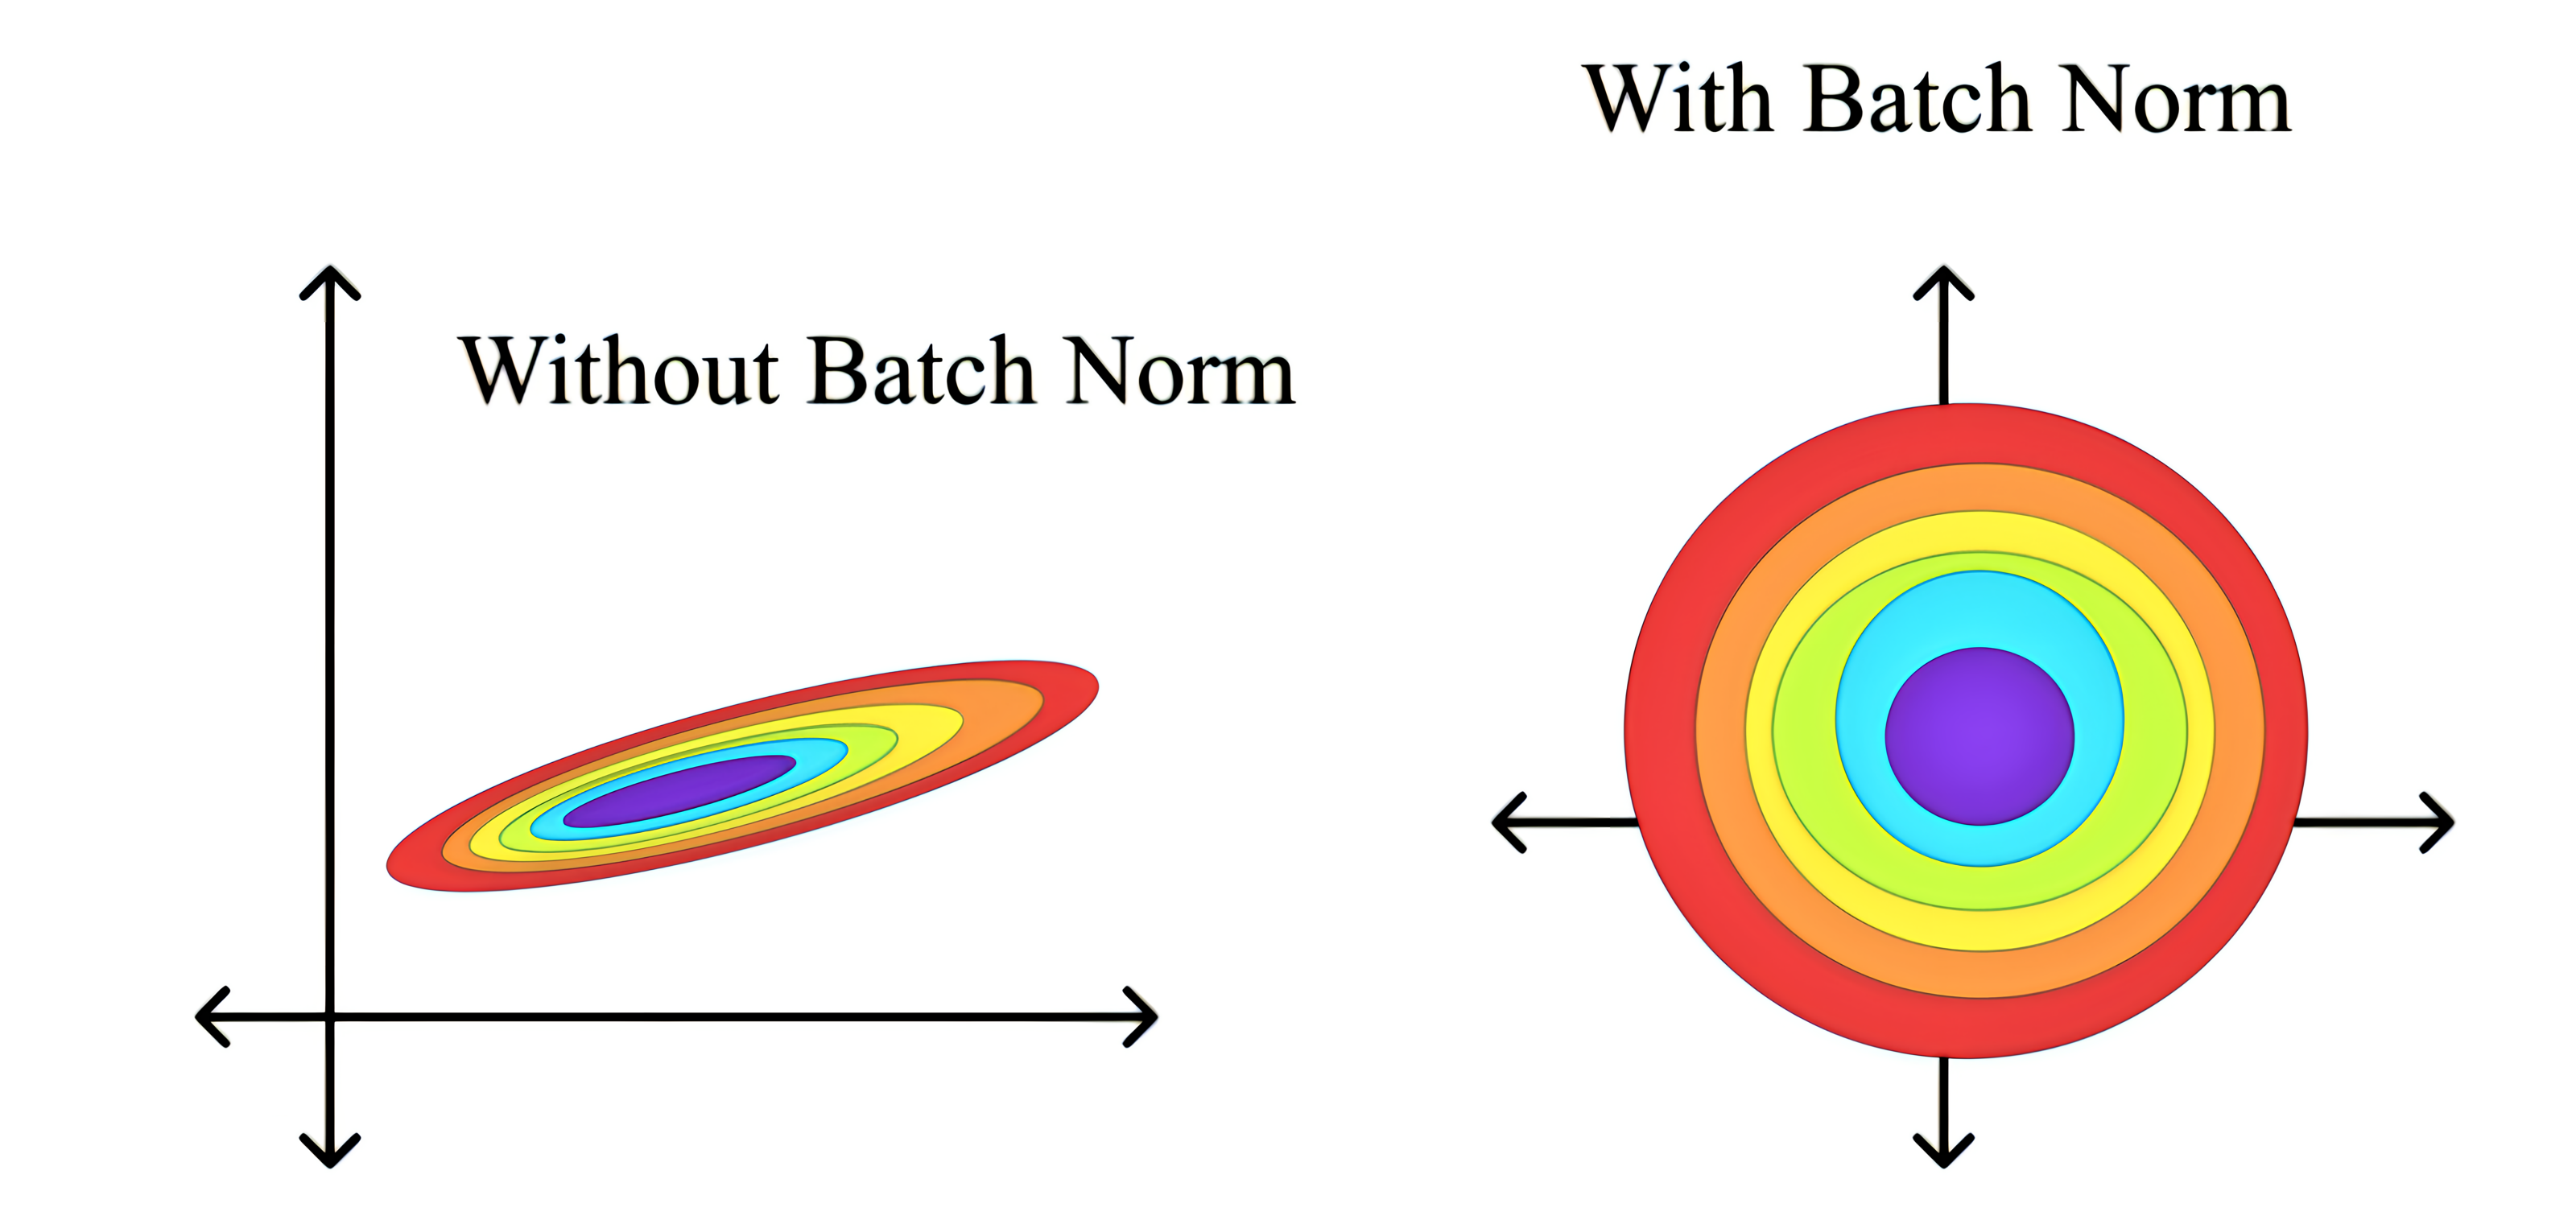
\includegraphics[width=0.85\textwidth]{pic/BatchNorm_Effect.png}
        \caption{Using Batch Normalization causes the optimization space to become smoother. \href{https://www.linkedin.com/pulse/ways-improve-your-deep-learning-model-batch-adam-albuquerque-lima}{\textcolor{orange}{\textbf{Source}}}}
        \label{fig:BN_Effect1}
    \end{figure}

\end{frame}

\subsection{Why Batch Normalization?}

\begin{frame}{Why Batch Normalization?}

    \textcolor{blue}{\textbf{Problem: Internal Covariate Shift}}

\begin{itemize}

    \item \textbf{Definition:} During training, as the parameters of earlier layers change, the distribution of inputs to deeper layers shifts, which slows down learning.
    \item \textbf{Impact:} This shift makes the network slower to train and requires careful tuning of the learning rate.
    \item \textbf{Example:} Imagine training a deep network where the input scale and distribution to each layer are constantly changing, making convergence harder to achieve.

\end{itemize}

\end{frame}

\begin{frame}{Why Batch Normalization?}

    \textcolor{blue}{\textbf{Batch Normalization Solution}}
    
    \begin{itemize}

    \item \textbf{Goal:} Normalize the inputs to each layer so that the mean is close to 0 and the variance is close to 1.
    \item \textbf{How it helps:} This stabilization of the learning process allows for higher learning rates and often leads to faster convergence.
    \item \textbf{Additional Benefits:}
        \begin{itemize}
        \item Reduces sensitivity to weight initialization.
        \item Mitigates vanishing and exploding gradient problems in deep neural networks.
        \end{itemize}


    \end{itemize}
\end{frame}

\begin{frame}{Magic Effect of Batch Normalization}

    \textcolor{blue}{\textbf{Magic Effect!}}
    
    \begin{itemize}
            \item Batch Normalization helps the network train faster and achieve higher accuracy.
            \item Batch Normalization \textbf{makes the distribution more stable} and reduces the internal covariate shift.
    \end{itemize}

        \begin{figure}
        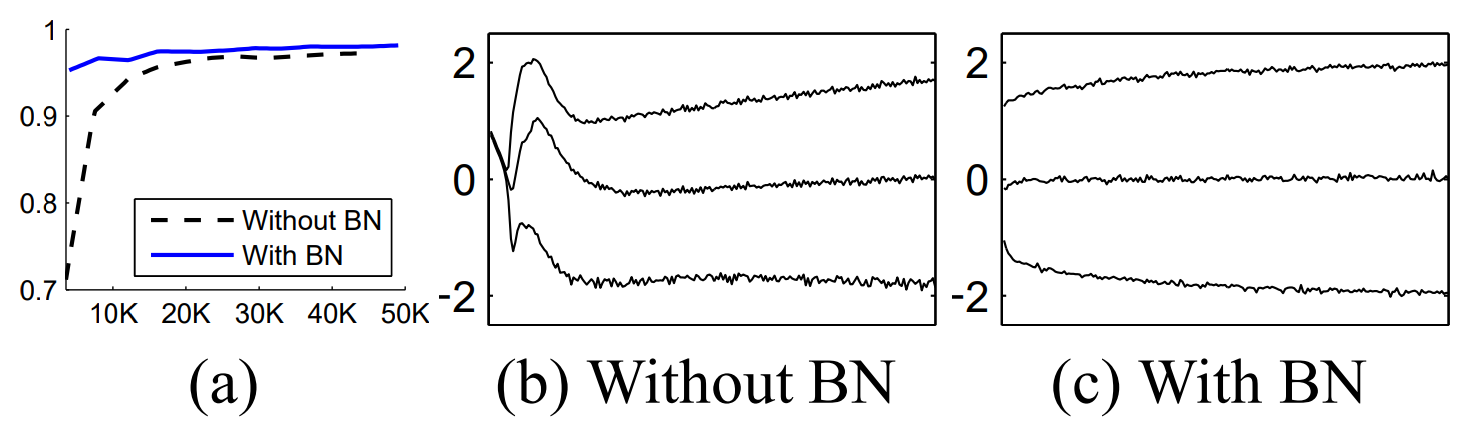
\includegraphics[width=0.7\textwidth]{pic/BN.png}
        \caption{(a) The test accuracy of the MNIST network trained with and without Batch Normalization, vs the number of training steps. (b, c) The evolution of input distributions to a typical sigmoid, over the course of training, shown as {15, 50, 85}th percentiles [1].}
        \label{fig:BN_Effect}
    \end{figure}
\end{frame}


\subsection{How Batch Normalization Works}

\begin{frame}{How Batch Normalization Works}

    \textcolor{blue}{\textbf{Process Overview}}
    
    \begin{itemize}

        \item  For each mini-batch during training, batch normalization normalizes the inputs to a layer by adjusting their mean and variance.

    \end{itemize}
\end{frame}

% Frame 1: Steps 1 and 2
\begin{frame}{How Batch Normalization Works}
    \textcolor{blue}{\textbf{Steps in Batch Normalization}}
    
    \begin{enumerate}[<+-| alert@+>] % stepwise alerts
        \item \textbf{Compute the Mean and Variance} 
              \newline
              For a given mini-batch, compute the mean $\mu_B$ and variance $\sigma_B^2$ of the inputs:
    
              \[
               \mu_B = \frac{1}{m} \sum_{i=1}^{m} x_i, \quad \sigma_B^2 = \frac{1}{m} \sum_{i=1}^{m} (x_i - \mu_B)^2
              \]
        \item \textbf{Normalize the Inputs}
        \newline
        Subtract the mean and divide by the standard deviation to get normalized activations:

        \[
        \hat{x}_i = \frac{x_i - \mu_B}{\sqrt{\sigma_B^2 + \epsilon}}
        \]

        where $\epsilon$ is a small constant added for numerical stability.
    \end{enumerate}
\end{frame}

% Frame 2: Step 3
\begin{frame}{How Batch Normalization Works (Continued)}
    \textcolor{blue}{\textbf{Steps in Batch Normalization}}
    
    % Resume the enumeration from step 3
    \begin{enumerate}[<+-| alert@+>] % stepwise alerts
        \setcounter{enumi}{2} % Set the counter to continue from step 3
        \item \textbf{Scale and Shift}
        \newline
        After normalization, introduce learnable parameters $\gamma$ and $\beta$ that allow the model to scale and shift the normalized output:
    
        \[
            y_i = \gamma \hat{x}_i + \beta
        \]

        This ensures that the model can recover the original data distribution if needed.
    \end{enumerate}
\end{frame}

\begin{frame}{How Batch Normalization Works}

    \textcolor{blue}{\textbf{Inference Mode:}} {\textbf{\textcolor{red}{Hint!!!}}}
    
    \begin{itemize}

        \item During inference (when predicting new data), batch statistics (mean and variance) are replaced with moving averages collected during training.

    \end{itemize}
\end{frame}

\begin{frame}
    \frametitle{Effect of Batch Normalization on Gradients}

    The main benefit of batch normalization is that it reduces the dependency of the gradient on the scale of the input and parameters:

    \begin{equation}
        \frac{\partial \mathcal{L}}{\partial x} = \frac{\partial \mathcal{L}}{\partial y} \cdot \frac{\partial y}{\partial \hat{x}} \cdot \frac{\partial \hat{x}}{\partial x}
    \end{equation}

    Where:
    \begin{itemize}
        \item \centering \(\frac{\partial y}{\partial \hat{x}} = \gamma\) \\
        \item \(\frac{\partial \hat{x}}{\partial x} = \frac{1}{\sqrt{\sigma_{\mathcal{B}}^2 + \epsilon}}\)
    \end{itemize}

    Thus, the gradient becomes:
    \begin{equation}
        \frac{\partial \mathcal{L}}{\partial x} = \frac{\gamma}{\sqrt{\sigma_{\mathcal{B}}^2 + \epsilon}} \cdot \frac{\partial \mathcal{L}}{\partial y}
    \end{equation}
\end{frame}

\begin{frame}
    \frametitle{How Batch Normalization Smooth the Cost Surface}

    The smoothing effect of batch normalization can be understood by observing how it constrains the gradient magnitudes. The expression shows that:
    \begin{equation}
        \frac{\partial \mathcal{L}}{\partial x} \text{ is scaled by } \frac{1}{\sqrt{\sigma_{\mathcal{B}}^2 + \epsilon}}
    \end{equation}

    This consistent scaling leads to a smoother loss surface because:
    \begin{itemize}
        \item It stabilizes the gradient flow, ensuring controlled optimization step sizes.
        \item Reduces the risk of large oscillations or abrupt changes in the loss landscape.
        \item Makes the optimization process less likely to be trapped in local minima or saddle points.
    \end{itemize}
\end{frame}


\subsection{Batch Normalization Pros \& Cons}

\begin{frame}{Batch Normalization Pros}

    \textcolor{green}{\textbf{Pros}}
    
    \begin{itemize}

        \item \textbf{Faster Convergence:}  Empirical results support that models with batch normalization converge faster and achieve higher accuracy, even with higher learning rates.
        \item \textbf{Reduced Sensitivity to  Weight Initialization:} Helps mitigate the dependency on careful weight initialization.
        \item \textbf{Acts as Regularization:} Batch normalization can help reduce overfitting.
        \item \textbf{Reduces Vanishing/Exploding Gradients:} Helps maintain stable gradients throughout deep networks.


    \end{itemize}
\end{frame}

\begin{frame}{Batch Normalization Pros}

    \textcolor{blue}{\textbf{Why Using Batch Normalization Reduces Sensitivity to Weight Initialization?}}

    \begin{figure}[h]
        \centering
        \subfigure[]{
            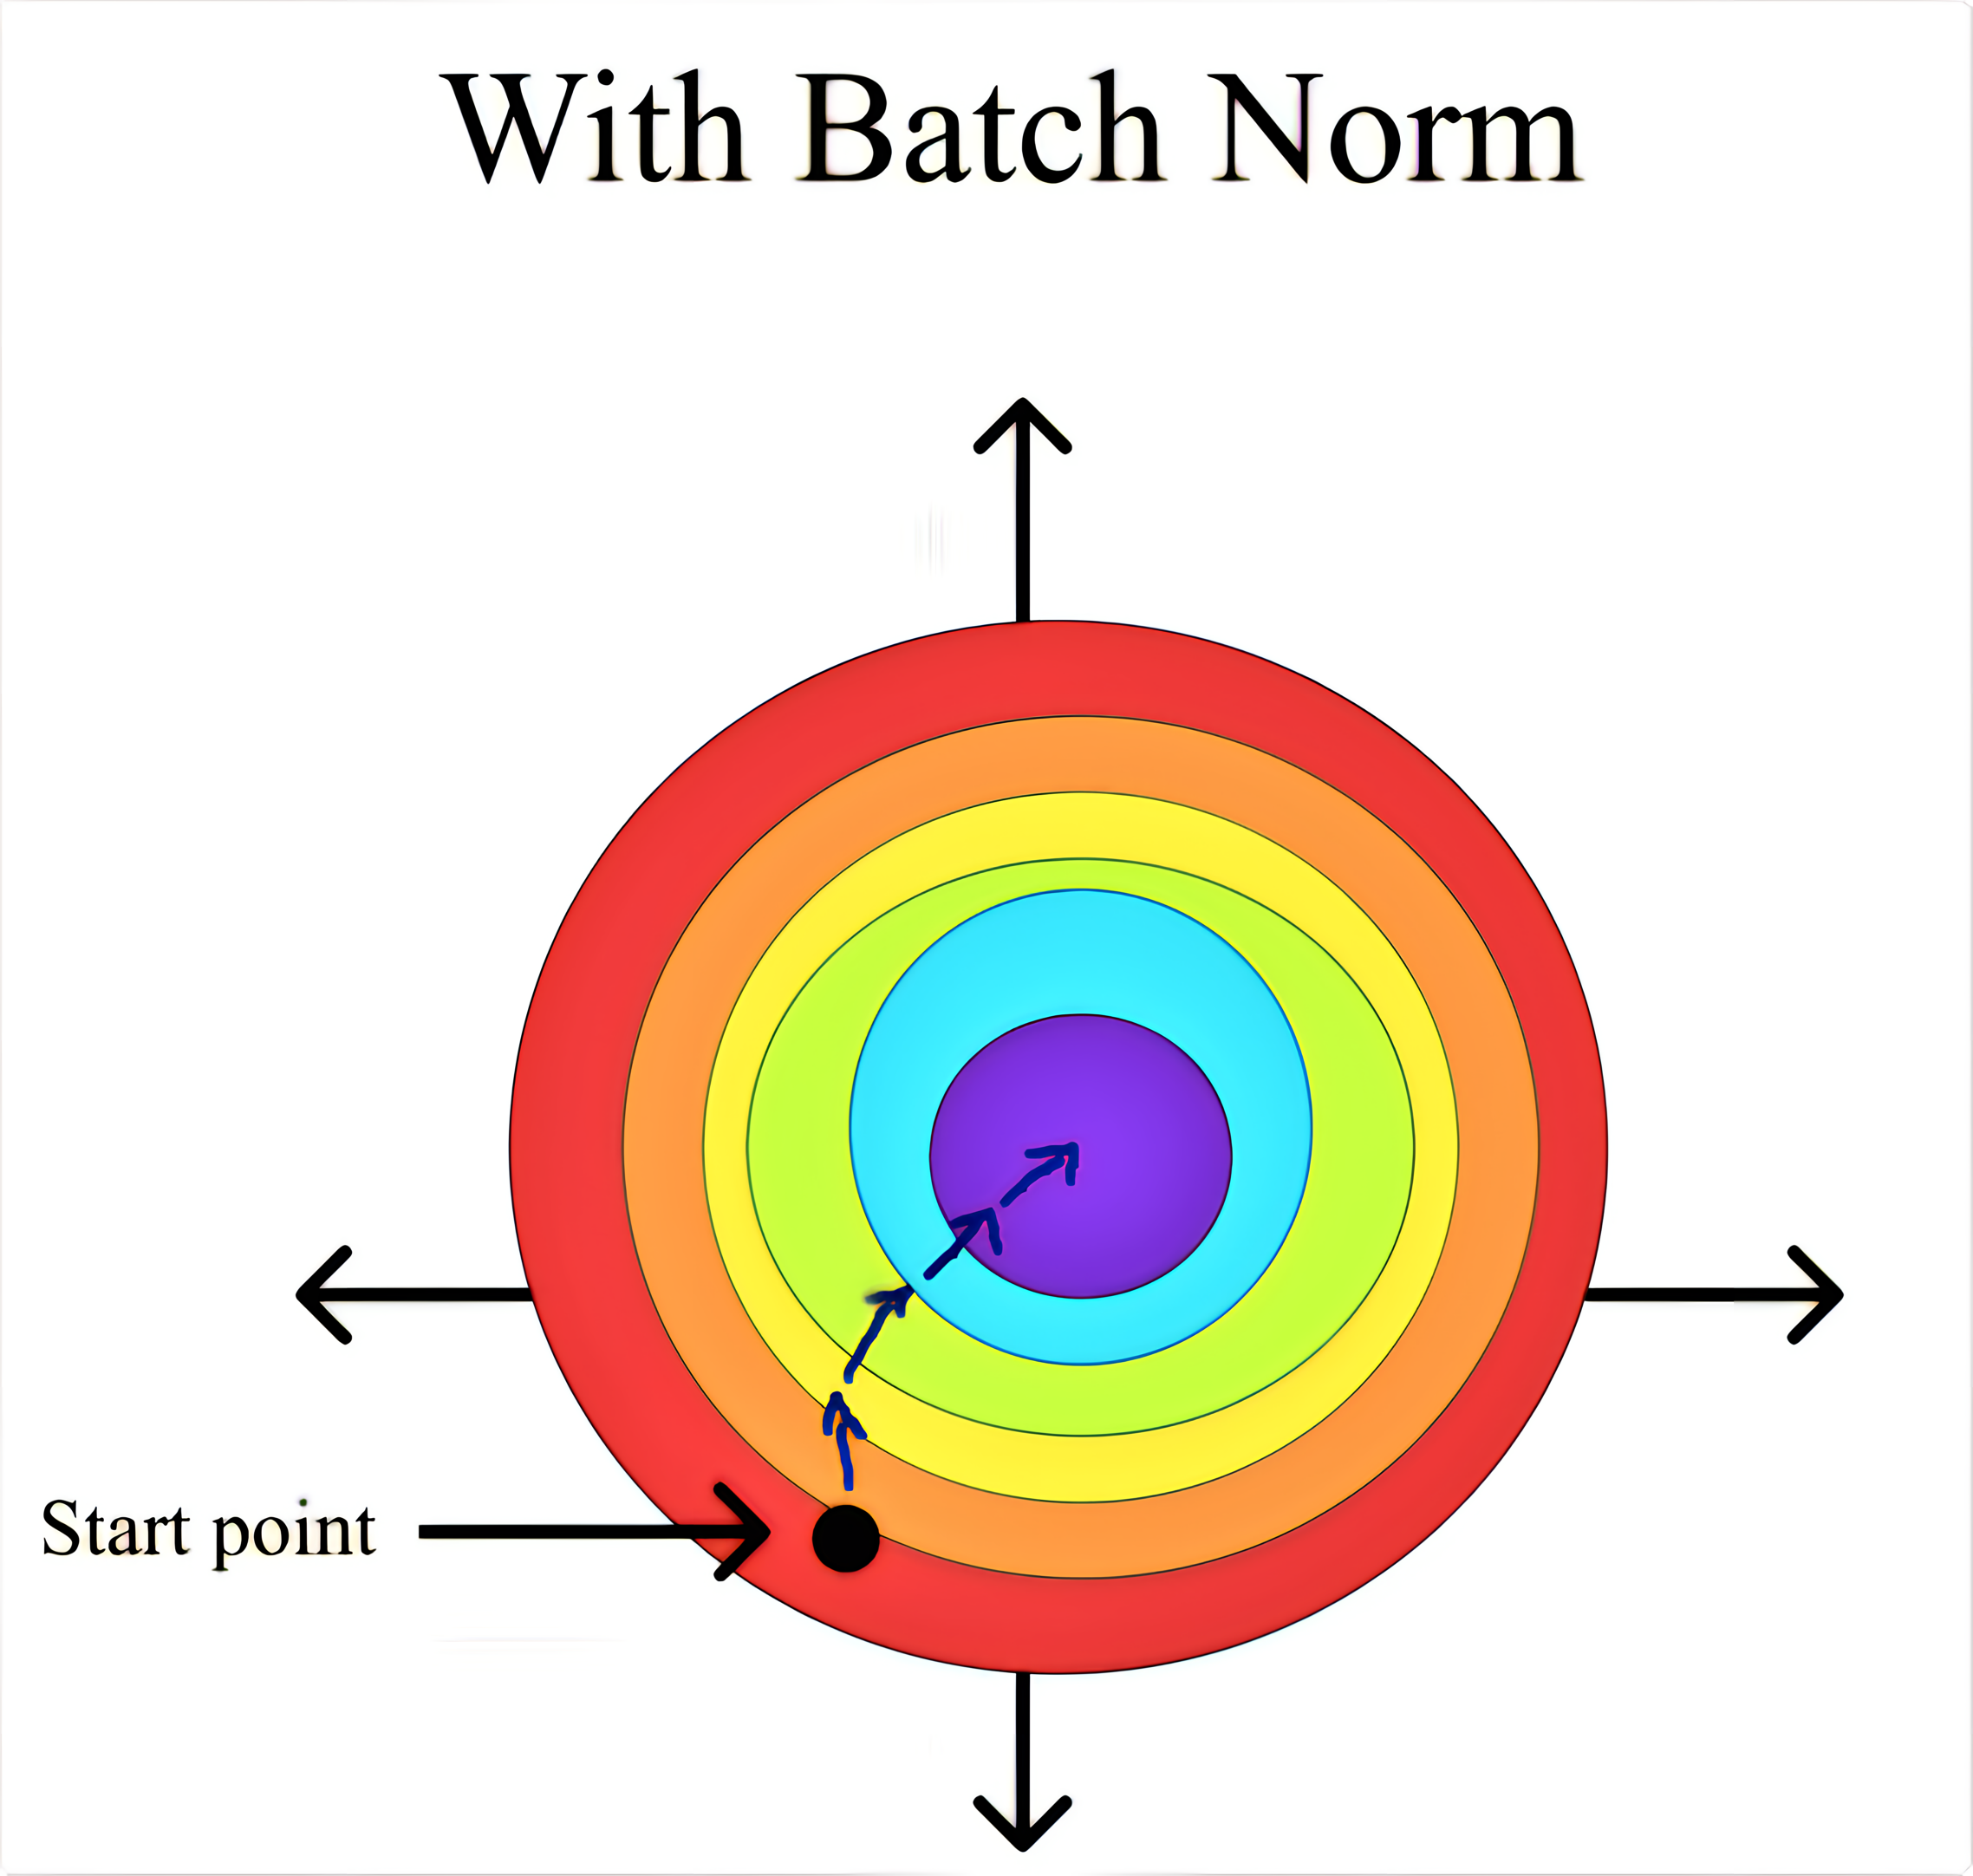
\includegraphics[width=0.3\textwidth]{pic/BN1.png}
            \label{fig:BN_Pros1}
        }
        \subfigure[]{
            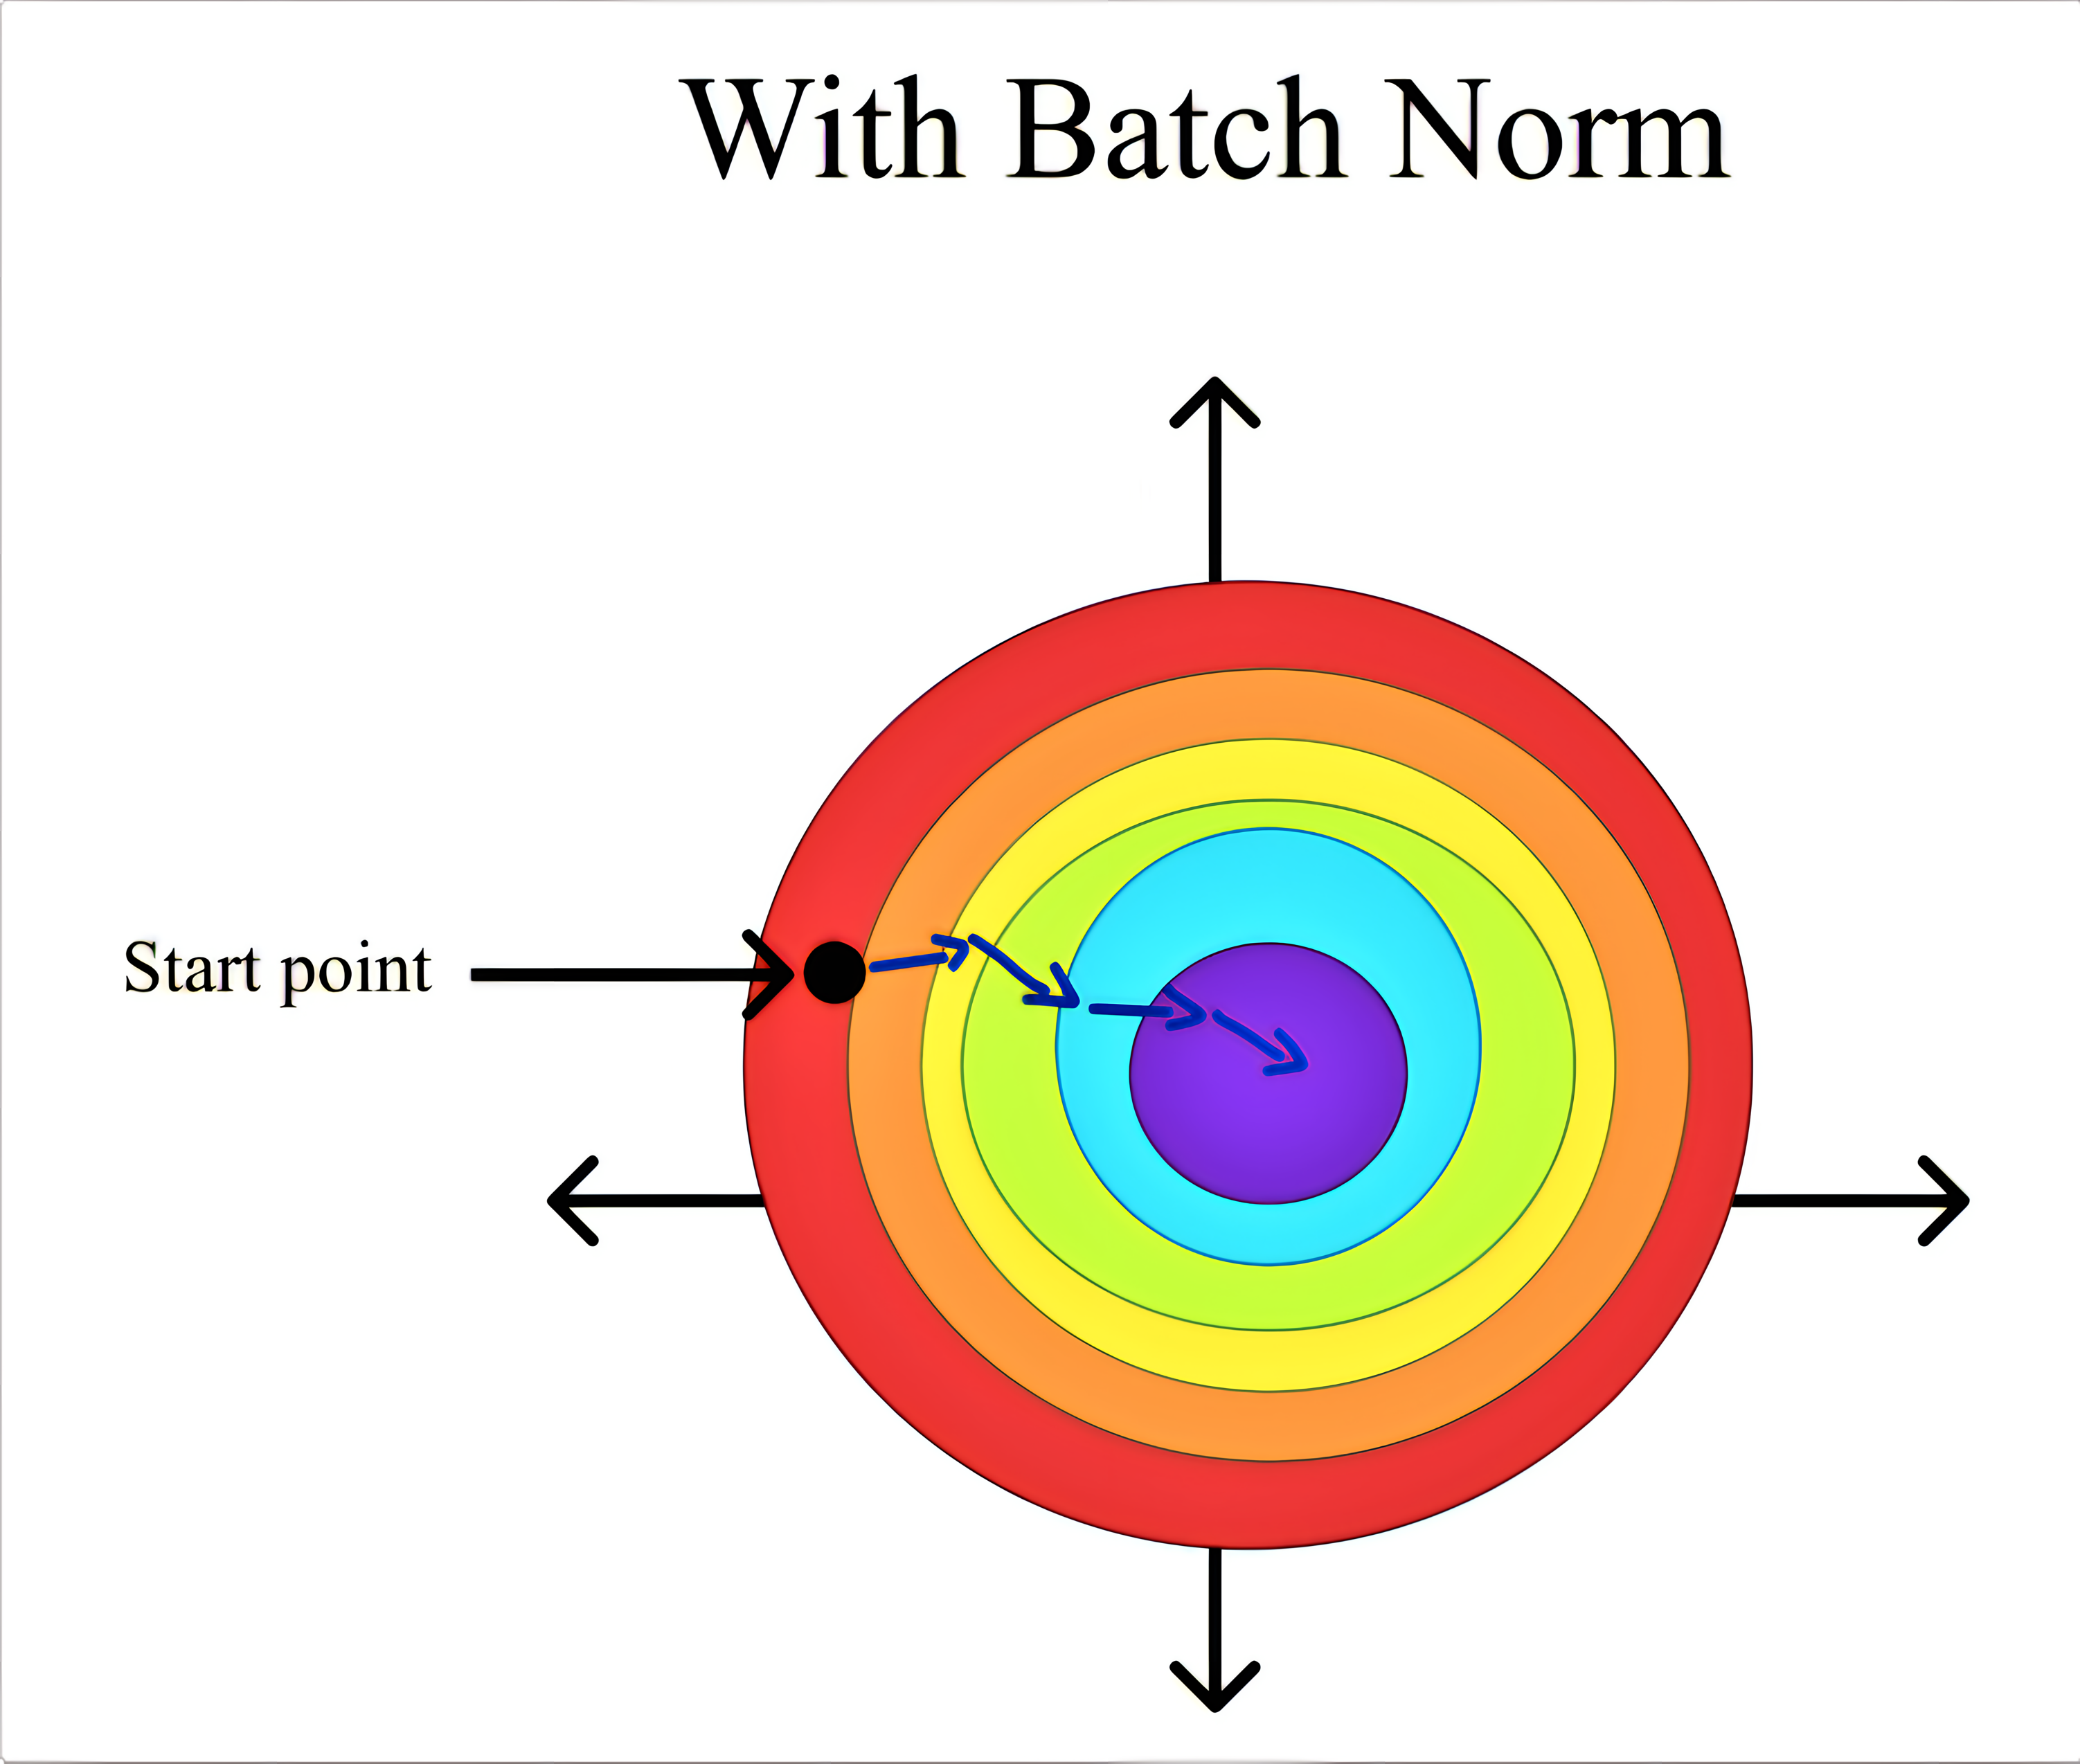
\includegraphics[width=0.33\textwidth]{pic/BN2.png}
            \label{fig:BN_Pros2}
        }
        \caption{Start point doesn't matter! \href{https://www.linkedin.com/pulse/ways-improve-your-deep-learning-model-batch-adam-albuquerque-lima}{\textcolor{orange}{\textbf{Source}}}}
    \end{figure}
\end{frame}

\begin{frame}{Batch Normalization Pros}

    \textcolor{blue}{\textbf{Why Using Batch Normalization Reduces Sensitivity to Weight Initialization?}}
    \begin{itemize}

        \item Batch normalization decreases the importance of initial weights because makes optimization space smoother, \\ so \textcolor{green}{doesn’t matter where you start}, you will get to the minimal point more or less with the same quantity of iterations in every start point.


    \end{itemize}
\end{frame}

\begin{frame}{Batch Normalization Cons}

    \textcolor{red}{\textbf{Cons}}
    
    \begin{itemize}

        \item \textbf{Batch Size Sensitivity:} Performance can depend on batch size, and very small batches may not provide stable statistics.
        \item \textbf{Computational Overhead:} Adds extra computation during training.
        \item \textbf{Behavior During Inference:} The shift from batch statistics to moving averages during inference may lead to slight discrepancies.

    \end{itemize}
\end{frame}

\subsection{Batch Normalization in Practice}

% \begin{frame}{Batch Normalization in Practice}

%     \textcolor{blue}{\textbf{Where to Apply}}
    
%     \begin{itemize}

%         \item \textbf{Typical Location:} Apply after the linear transformation (e.g., after a dense or convolutional layer) but before the activation function
%         \item \textbf{Layer Placement:}
%             \newline
%             Dense layer -> Batch Normalization -> Activation function
%             Conv layer -> Batch Normalization -> Activation function

%     \end{itemize}
% \end{frame}

\begin{frame}{Batch Normalization in Practice}

    \textcolor{blue}{\textbf{Where to Apply}}
    
    \begin{itemize}
        \item \textbf{Typical Location:} Apply after the linear transformation (e.g., after a dense or convolutional layer) but before the activation function.
        \item \textbf{Layer Placement:}
            \newline
\begin{center}
    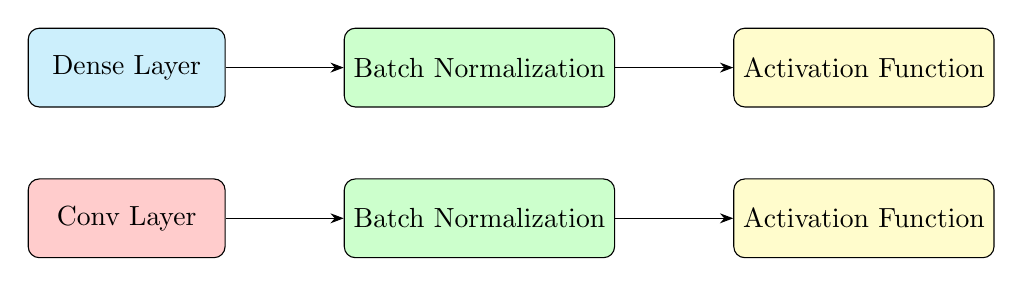
\begin{tikzpicture}[
        node distance=0.9cm and 1.5cm, % Distance between nodes
        every node/.style={draw, rounded corners, text centered, minimum height=1cm, minimum width=2.5cm}, % Style for every node
        bn/.style={fill=green!20}, % Style for batch normalization nodes
        conv/.style={fill=red!20}, % New style for conv layer
        dense/.style={fill=cyan!20}, % New style for dense layer
        act/.style={fill=yellow!20}, % New style for activation functions
        ->, >=Stealth % Arrow styles
    ]

        % Define nodes for the first path
        \node[dense] (dense) {Dense Layer};
        \node[bn] (bn1) [right=of dense] {Batch Normalization};
        \node[act] (act1) [right=of bn1] {Activation Function};

        % Define nodes for the second path
        \node[conv] (conv) [below=of dense] {Conv Layer};
        \node[bn] (bn2) [right=of conv] {Batch Normalization};
        \node[act] (act2) [right=of bn2] {Activation Function};

        % Draw arrows between nodes
        \draw[->] (dense) -- (bn1);
        \draw[->] (bn1) -- (act1);

        \draw[->] (conv) -- (bn2);
        \draw[->] (bn2) -- (act2);

    \end{tikzpicture}
\end{center}
    \end{itemize}
    
\end{frame}



\subsection{Closing Takeaways on Batch Normalization}

\begin{frame}{Batch Normalization in Practice}
    
    \begin{itemize}

        \item \textbf{Key Point:} Batch normalization has become an essential tool in deep learning due to its ability to stabilize and accelerate training, while also acting as a form of regularization.
        \item \textbf{Impact on Training:} Allows deeper networks to be trained more efficiently and with fewer hyperparameter tuning efforts.

    \end{itemize}
\end{frame}


\section{References}

\begin{frame}[allowframebreaks]
    \bibliography{ref}
    \bibliographystyle{ieeetr}
    \nocite{*} % used here because no citation happens in slides
    % if there are too many try use:
    % \tiny\bibliographystyle{alpha}
\end{frame}


\begin{frame}
    \begin{center}
        {\Huge Any Questions?}
    \end{center}
\end{frame}

\end{document}